\documentclass[aspectratio=169, 10pt]{beamer}

\usepackage{bm} % bold math
\usepackage{fontspec}
\usepackage{minted}
\usepackage{pgf-pie}
\usepackage{tikz}

% Custom commands and environments
\makeatletter
\newcommand\version[1]{\renewcommand\@version{#1}}
\newcommand\@version{}
\def\insertversion{\@version}

\newcommand\course[1]{\renewcommand\@course{#1}}
\newcommand\@course{}
\def\insertcourse{\@course}

\newcommand\coursetitle[1]{\renewcommand\@coursetitle{#1}}
\newcommand\@coursetitle{}
\def\insertcoursetitle{\@coursetitle}

\newcommand\lecturenumber[1]{\renewcommand\@lecturenumber{#1}}
\newcommand\@lecturenumber{}
\def\insertlecturenumber{\@lecturenumber}
\makeatother

\newcommand{\slidetitle}[1]{{\xbseries \large \structure{#1}} \bigskip}
\newcommand{\term}[1]{{\color{blue} #1}}
\newcommand{\leftspace}{\hspace{1em}}
\newcommand{\inlinearrow}{
  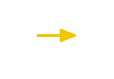
\begin{tikzpicture}[baseline]
    \node [anchor=base] (x) {};
    \draw [rawarrow] (x.mid west) -- ($(x.mid west) + (2em,0)$);
  \end{tikzpicture}
}

\newenvironment{slide}
{\begin{frame}[fragile,environment=slide]\vskip0pt plus 1filll}
{\vskip0pt plus 1filll\end{frame}}

% LaTeX

\setlength{\leftmargini}{1em}

% Common Information

\author{Jon Eyolfson}
\course{ECE 353}
\coursetitle{Systems Software}
\date{2024 Winter}

% fontspec

\defaultfontfeatures{Ligatures=TeX}
% \setmainfont{Domine}
\setsansfont{Inter}[
  FontFace={ul}{n}{Font=*-Thin},
  FontFace={el}{n}{Font=*-ExtraLight},
  FontFace={l}{n}{Font=*-Light},
  FontFace={sb}{n}{Font=*-SemiBold},
  FontFace={eb}{n}{Font=*-ExtraBold},
  FontFace={xb}{n}{Font=*-Black},
]
\setmonofont[Contextuals=AlternateOff, Ligatures=TeXOff]{Iosevka}[
  FontFace={xb}{n}{Font=*-Heavy},
]

%% Font Weights

\DeclareRobustCommand{\ulseries}{\fontseries{ul}\selectfont}
\DeclareTextFontCommand{\textul}{\ulseries}
\DeclareRobustCommand{\elseries}{\fontseries{el}\selectfont}
\DeclareTextFontCommand{\textel}{\elseries}
\DeclareRobustCommand{\lseries}{\fontseries{l}\selectfont}
\DeclareTextFontCommand{\textl}{\lseries}
\DeclareRobustCommand{\sbseries}{\fontseries{sb}\selectfont}
\DeclareTextFontCommand{\textsb}{\sbseries}
\DeclareRobustCommand{\ebseries}{\fontseries{eb}\selectfont}
\DeclareTextFontCommand{\texteb}{\ebseries}
\DeclareRobustCommand{\xbseries}{\fontseries{xb}\selectfont}
\DeclareTextFontCommand{\textxb}{\xbseries}

% tikz

\usetikzlibrary{
  arrows,
  arrows.meta,
  automata,
  backgrounds,
  calc,
  decorations.pathreplacing,
  matrix,
  positioning,
  overlay-beamer-styles,
  shapes,
  shapes.multipart,
  tikzmark,
}

\tikzstyle{rawarrow} = [
  -{Latex[round]},
  line width=1pt,
  yellow,
  shorten >=3pt,
  shorten <=3pt,
  font=\small,
  text=black,
]

\tikzstyle{arrow} = [
  -{Latex[round]},
  line width=1pt,
  yellow,
  shorten >=3pt,
  shorten <=3pt,
  transform canvas={yshift=3pt},
  font=\small,
  text=black,
]

\newcommand{\tikzmarkcoord}[1]{([yshift=3pt]pic cs:#1)}

% minted

\setminted{style=eyolfson, fontsize=\small, escapeinside=||}
\setmintedinline{fontsize=\normalsize}

% hyperref

\hypersetup{colorlinks, urlcolor=blue}

% beamer
\setbeamersize{text margin left=16mm, text margin right=16mm}
\setbeamertemplate{itemize items}[circle]
\setbeamercolor{item}{fg=black}
\setbeamercolor{structure}{fg=darkblue}
\setbeamerfont{frametitle}{series=\bfseries, parent=structure}
\setbeamertemplate{navigation symbols}{}
\setbeamertemplate{headline}{}
\setbeamertemplate{footline}{
  \begin{tikzpicture}[
    remember picture,
    overlay,
    shift={(current page.south west)},
  ]
    \path [fill=gray] (144mm, 0) -- (160mm, 16mm) -- (160mm, 0);
    \node [inner sep=3.5mm, outer sep=0, text=black, anchor=base east,
           align=right, yshift=3.5mm]
          at (current page.south east) {\ttfamily \small \insertframenumber{}};
  \end{tikzpicture}
}
\setbeamertemplate{title page}{
  \begin{tikzpicture}[
    remember picture,
    overlay,
    shift={(current page.south west)},
    background rectangle/.style={fill=darkblue},
    show background rectangle,
  ]
    \node [anchor=center, align=center, text=white, text width=40mm, scale=3.2]
          at (\paperwidth / 2, \paperheight * 2 / 3)
          {\xbseries \inserttitle{}};
    \node [anchor=base west, align=left, inner sep=0, text=white, yshift=2.5mm]
          at (16mm, \paperheight / 3)
          {\insertdate{} \insertcourse{}: \insertcoursetitle{}};
    \node [anchor=base west, align=left, inner sep=0, text=white, yshift=-2.5mm]
          at (16mm, \paperheight / 3)
          {\insertauthor};
    \node [anchor=base east, align=right, inner sep=0, text=white, yshift=2.5mm]
          at (144mm, \paperheight / 3)
          {Lecture \insertlecturenumber{}};
    \node [anchor=base east, align=right, inner sep=0, text=white,
           yshift=-2.5mm]
          at (144mm, \paperheight / 3)
          {\ttfamily \insertversion{}};
    \node [align=center, anchor=south, inner sep=0, text=white, yshift=3.5mm]
          (license) at (\paperwidth / 2, 0)
          {\fontsize{7pt}{7pt}\selectfont This  work is licensed under a
           \href{http://creativecommons.org/licenses/by-sa/4.0/}
                {\color{lightblue} Creative Commons Attribution-ShareAlike 4.0
                 International License}};
  \end{tikzpicture}
}

% xcolor

%% Primary Colour

\definecolor{pantone655}{RGB}{0, 42, 92} % #002a5c
\colorlet{darkblue}{pantone655}

%% Secondary Colours

\definecolor{pantone633}{RGB}{0, 139, 176} % #008bb0
\colorlet{blue}{pantone633}

\definecolor{pantonewarmred}{RGB}{220, 70, 51} % #dc4633
\colorlet{red}{pantonewarmred}

\definecolor{pantone3285}{RGB}{0, 161, 137} % #00a189
\colorlet{cyan}{pantone3285}

\definecolor{pantone7722}{RGB}{13, 83, 77} % #0d534d
\colorlet{darkcyan}{pantone7722}

\definecolor{pantone376}{RGB}{141, 191, 46} % #8dbf2e
\colorlet{green}{pantone376}

\definecolor{pantone2613}{RGB}{109, 36, 122} % #6d247a
\colorlet{violet}{pantone2613}

\definecolor{pantone2985}{RGB}{111, 199, 234} % #6fc7ea
\colorlet{lightblue}{pantone2985}

\definecolor{pantone227}{RGB}{171, 19, 104} % #ab1368
\colorlet{magenta}{pantone227}

\definecolor{pantone7406}{RGB}{241, 197, 0} % #f1c500
\colorlet{yellow}{pantone7406}

%% Neutrals

\definecolor{pantonecoolgray2}{RGB}{208, 209, 201} % #d0d1c9
\colorlet{gray}{pantonecoolgray2}


\lecturenumber{14}
\title{Priority Scheduling and Memory Mapping}
\version{2.0.0}

\begin{document}
  \begin{frame}[plain, noframenumbering]
    \titlepage
  \end{frame}

  \begin{slide}

    \slidetitle{Let's Explore a Dynamic Priority Scheduling}

    This may also be called: Feedback Scheduling
    \medskip

    We let the algorithm manage the priorities

    \leftspace{}We use set time slices, and measure CPU usage
    \medskip

    Increase the priority of processes that don't use their time slice
    \medskip

    Decrease the priority of processes that use their full time slice

  \end{slide}

  \begin{slide}

    \slidetitle{We Pick the Lowest Number as Highest Priority}

    Each process gets assigned a priority when started, $P_n$
    \medskip

    Pick the lowest priority number to schedule, if it yields, pick the
    next lowest number

    \leftspace{}Break ties with arrival order

    \leftspace{}If a lower priority number becomes ready, switch to it
    \medskip

    Record how much time each process executes for in this priority interval,
    $\mathsf{C_n}$

    \leftspace{}Timer interrupts still occur
    \medskip
  
    At the end of the priority interval, update the priority of each process
    with:

    \leftspace{}$\mathsf{P_n =  \frac{P_n}{2} + C_n}$ 

    \leftspace{}and reset the value of $\mathsf{C_n}$ back to 0

  \end{slide}

  \begin{slide}

    \slidetitle{Assume All Processes Have an Initial Priority of 0}

    Assume we have 4 processes ready to execute arriving in order: X, Y, A, B

    \leftspace{}A and B are CPU bound processes

    \leftspace{}X and Y are I/O bound processes that execute for 1 and
    block for 5

    Timer interrupts occur every 1, and each time slice is 10, priority interval
    is 10
    \medskip

    What is the scheduling? (each box is a timer interrupt)

    \begin{center}
      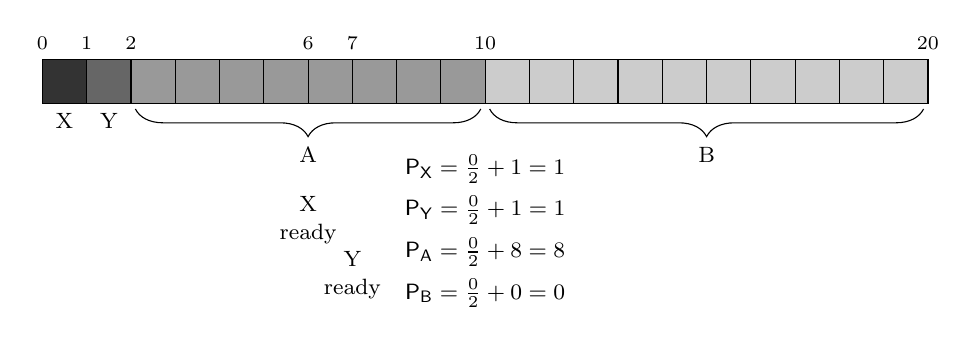
\begin{tikzpicture}[scale=0.8]

        \fill [black!80, visible on=<2->] (0,0) rectangle (2em, 2em);

        \fill [black!60, visible on=<3->] (2em,0) rectangle (4em, 2em);

        \fill [black!40, visible on=<4->] (4em,0) rectangle (20em, 2em);

        \fill [black!20, visible on=<8->] (20em,0) rectangle (40em, 2em);

        \draw (0,0) rectangle (40em,2em);

        \foreach \i in {1,...,19} {
          \draw [shorten >=0] (\i * 2em, 0) -- (\i * 2em, 2em);
        }

        \node [anchor=south] at (0em, 2em) {\scriptsize 0};
        \node [anchor=south, visible on=<2->] at (2em, 2em) {\scriptsize 1};
        \node [anchor=south, visible on=<3->] at (4em, 2em) {\scriptsize 2};
        \node [anchor=south, visible on=<5->] at (12em, 2em) {\scriptsize 6};
        \node [anchor=south, visible on=<6->] at (14em, 2em) {\scriptsize 7};
        \node [anchor=south] at (20em, 2em) {\scriptsize 10};
        \node [anchor=south] at (40em, 2em) {\scriptsize 20};

        \node [anchor=north, yshift=-3em, visible on=<5->] at (12em, 0em)
              {\footnotesize X};
        \node [anchor=north, yshift=-4em, visible on=<5->] at (12em, 0em)
              {\footnotesize ready};

        \node [anchor=north, yshift=-5em, visible on=<6->] at (14em, 0em)
              {\footnotesize Y};
        \node [anchor=north, yshift=-6em, visible on=<6->] at (14em, 0em)
              {\footnotesize ready};

        \node [anchor=north, yshift=-1.5em, visible on=<7->] at (20em, 0em)
              {\footnotesize $\mathsf{P_X} = \frac{0}{2} + 1 = 1$};
        \node [anchor=north, yshift=-3em, visible on=<7->] at (20em, 0em)
              {\footnotesize $\mathsf{P_Y} = \frac{0}{2} + 1 = 1$};
        \node [anchor=north, yshift=-4.5em, visible on=<7->] at (20em, 0em)
              {\footnotesize $\mathsf{P_A} = \frac{0}{2} + 8 = 8$};
        \node [anchor=north, yshift=-6em, visible on=<7->] at (20em, 0em)
              {\footnotesize $\mathsf{P_B} = \frac{0}{2} + 0 = 0$};

        \node [anchor=north, visible on=<2->] at (1em, 0) {\footnotesize X};

        \node [anchor=north, visible on=<3->] at (3em, 0) {\footnotesize Y};

        \draw [decorate, decoration={brace,amplitude=10pt,mirror,raise=2pt},
               visible on=<4->]
              (4.2em,0) -- (19.8em,0)
              node [midway, below, anchor=north, yshift=-1.25em]
              {\footnotesize A};

        \draw [decorate, decoration={brace,amplitude=10pt,mirror,raise=2pt},
               visible on=<8->]
              (20.2em,0) -- (39.8em,0)
              node [midway, below, anchor=north, yshift=-1.25em]
              {\footnotesize B};
      \end{tikzpicture}
    \end{center}

  \end{slide}

  \begin{slide}

    \slidetitle{Now, Processes A and B have a Priority of 6 (others are 0)}

    Assume we have 4 processes ready to execute arriving in order: X, Y, A, B

    \leftspace{}A and B are CPU bound processes

    \leftspace{}X and Y are I/O bound processes that execute for 1 and
    block for 5

    Timer interrupts occur every 1, and each time slice is 10, priority interval
    is 10
    \medskip

    What is the scheduling? (each box is a timer interrupt)

    \begin{center}
      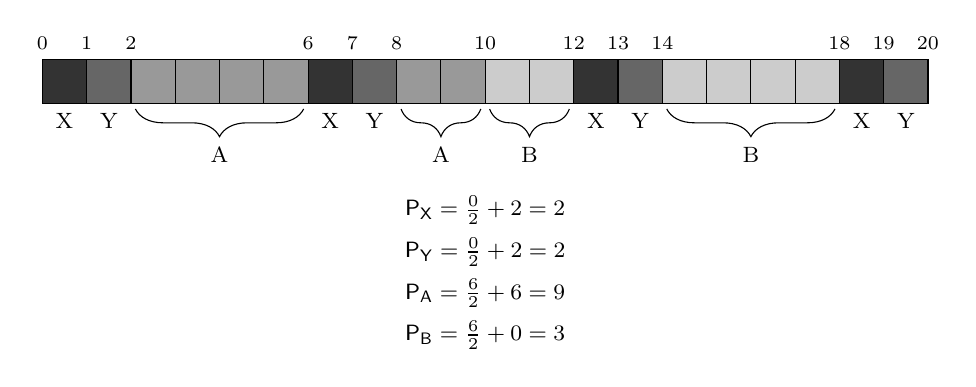
\begin{tikzpicture}[scale=0.8]

        \fill [black!80, visible on=<2->] (0,0) rectangle (2em, 2em);
        \fill [black!60, visible on=<3->] (2em,0) rectangle (4em, 2em);
        \fill [black!40, visible on=<4->] (4em,0) rectangle (12em, 2em);
        \fill [black!80, visible on=<5->] (12em,0) rectangle (14em, 2em);
        \fill [black!60, visible on=<6->] (14em,0) rectangle (16em, 2em);
        \fill [black!40, visible on=<7->] (16em,0) rectangle (20em, 2em);
        \fill [black!20, visible on=<9->] (20em,0) rectangle (24em, 2em);
        \fill [black!80, visible on=<10->] (24em,0) rectangle (26em, 2em);
        \fill [black!60, visible on=<11->] (26em,0) rectangle (28em, 2em);
        \fill [black!20, visible on=<12->] (28em,0) rectangle (36em, 2em);
        \fill [black!80, visible on=<13->] (36em,0) rectangle (38em, 2em);
        \fill [black!60, visible on=<14->] (38em,0) rectangle (40em, 2em);

        \draw (0,0) rectangle (40em,2em);

        \foreach \i in {1,...,19} {
          \draw [shorten >=0] (\i * 2em, 0) -- (\i * 2em, 2em);
        }

        \node [anchor=south] at (0em, 2em) {\scriptsize 0};
        \node [anchor=south, visible on=<2->] at (2em, 2em) {\scriptsize 1};
        \node [anchor=south, visible on=<3->] at (4em, 2em) {\scriptsize 2};
        \node [anchor=south, visible on=<4->] at (12em, 2em) {\scriptsize 6};
        \node [anchor=south, visible on=<5->] at (14em, 2em) {\scriptsize 7};
        \node [anchor=south, visible on=<6->] at (16em, 2em) {\scriptsize 8};
        \node [anchor=south, visible on=<9->] at (24em, 2em) {\scriptsize 12};
        \node [anchor=south, visible on=<10->] at (26em, 2em) {\scriptsize 13};
        \node [anchor=south, visible on=<11->] at (28em, 2em) {\scriptsize 14};
        \node [anchor=south, visible on=<12->] at (36em, 2em) {\scriptsize 18};
        \node [anchor=south, visible on=<13->] at (38em, 2em) {\scriptsize 19};
        \node [anchor=south] at (20em, 2em) {\scriptsize 10};
        \node [anchor=south] at (40em, 2em) {\scriptsize 20};

        \node [anchor=north, yshift=-3em, visible on=<8->] at (20em, 0em)
              {\footnotesize $\mathsf{P_X} = \frac{0}{2} + 2 = 2$};
        \node [anchor=north, yshift=-4.5em, visible on=<8->] at (20em, 0em)
              {\footnotesize $\mathsf{P_Y} = \frac{0}{2} + 2 = 2$};
        \node [anchor=north, yshift=-6em, visible on=<8->] at (20em, 0em)
              {\footnotesize $\mathsf{P_A} = \frac{6}{2} + 6 = 9$};
        \node [anchor=north, yshift=-7.5em, visible on=<8->] at (20em, 0em)
              {\footnotesize $\mathsf{P_B} = \frac{6}{2} + 0 = 3$};

        \node [anchor=north, visible on=<2->] at (1em, 0) {\footnotesize X};

        \node [anchor=north, visible on=<3->] at (3em, 0) {\footnotesize Y};

        \draw [decorate, decoration={brace,amplitude=10pt,mirror,raise=2pt},
               visible on=<4->]
              (4.2em,0) -- (11.8em,0)
              node [midway, below, anchor=north, yshift=-1.25em]
              {\footnotesize A};

        \node [anchor=north, visible on=<5->] at (13em, 0) {\footnotesize X};

        \node [anchor=north, visible on=<6->] at (15em, 0) {\footnotesize Y};

        \draw [decorate, decoration={brace,amplitude=10pt,mirror,raise=2pt},
               visible on=<7->]
              (16.2em,0) -- (19.8em,0)
              node [midway, below, anchor=north, yshift=-1.25em]
              {\footnotesize A};

        \draw [decorate, decoration={brace,amplitude=10pt,mirror,raise=2pt},
               visible on=<9->]
              (20.2em,0) -- (23.8em,0)
              node [midway, below, anchor=north, yshift=-1.25em]
              {\footnotesize B};

        \node [anchor=north, visible on=<10->] at (25em, 0) {\footnotesize X};

        \node [anchor=north, visible on=<11->] at (27em, 0) {\footnotesize Y};

        \draw [decorate, decoration={brace,amplitude=10pt,mirror,raise=2pt},
               visible on=<12->]
              (28.2em,0) -- (35.8em,0)
              node [midway, below, anchor=north, yshift=-1.25em]
              {\footnotesize B};

        \node [anchor=north, visible on=<13->] at (37em, 0) {\footnotesize X};

        \node [anchor=north, visible on=<14->] at (39em, 0) {\footnotesize Y};
      \end{tikzpicture}
    \end{center}

  \end{slide}

  \begin{slide}
    
    \slidetitle{A 30B LLM on with Only 6.8 GB of RAM, how?}

    LLaMA is Meta's large language model, and this C++ implementation is
    efficient
    \medskip

    It's so efficient people are discussing how this is possible!

    \url{https://github.com/ggerganov/llama.cpp/discussions/638}

  \end{slide}

  \begin{slide}
    
    \slidetitle{We Can Control Our Processes' Virtual Memory}

    Memory map, or \texttt{mmap} is used to map files to a processes' virtual
    address space
    \medskip

    The pointer (virtual address) returned will allow you to access the file
    directly

    \leftspace{}There's no need for \texttt{read} and \texttt{write} system
    calls

  \end{slide}

  \begin{slide}
    
    \slidetitle{The \texttt{mmap} API}

    \texttt{mmap} takes 6 arguments:

    \begin{enumerate}
      \item \texttt{\bfseries void *addr}: suggested starting address
            (\texttt{NULL} means you don't care)
      \item \texttt{\bfseries size\_t length}: number of bytes to map
      \item \texttt{\bfseries int prot}: protection flags (read/write/execute)
      \item \texttt{\bfseries int flags}: mapping flags
            (shared/private/anonymous)

            \hspace{5em}  anonymous means the mapping isn't backed by a file
      \item \texttt{\bfseries int fd}: file descriptor to map (ignored for
            anonymous)
      \item \texttt{\bfseries off\_t offset}: offset to start the mapping (must
            be a multiple of page size)
    \end{enumerate}

  \end{slide}

  \begin{slide}
    
    \slidetitle{Let's See a \texttt{mmap} Example}

    Check out \texttt{lectures/14-priority-scheduling-and-memory-mapping} in the
    \texttt{materials} repository

  \end{slide}

  \begin{slide}
    
    \slidetitle{\texttt{mmap} Is Lazy}

    It just sets up the page tables, it doesn't actually read from the file
    \medskip

    It would create an invalid PTE during the \texttt{mmap} call
    \medskip

    The kernel uses the remaining bits of the PTE for bookkeeping

    \leftspace{}Where on the disk is this entry
    \medskip

    The first access to the page would generate a page fault

    \leftspace{}The kernel would then read from disk into memory
    \medskip

    This ensures only the used parts of the file get read

  \end{slide}

  \begin{slide}
    
    \slidetitle{Back to the Question}

    \url{https://github.com/ggerganov/llama.cpp/discussions/638}
    \medskip

    How does an approximately 20 GB file only use 6.8 GB of real memory?
    \medskip

    Hint: when you do model inference, the models are sparse (you don't use all
    of it)

  \end{slide}

  \begin{slide}
    
    \slidetitle{How Much Space Would the Kernel Need for Page Tables?}

    Someone posted you'd need 40 MB of page tables:

    \texttt{(20*(1024*1024*1024)/4096*8) / (1024*1024)}
    \medskip

    Someone clarified it's:

    \texttt{(20GB / 4KB Page size * 8 bytes per PTE) / 1KB}

    \leftspace{}(the 1KB at the end should be 1MB)
    \medskip

    Is this correct? Why or why not?

  \end{slide}

  \begin{slide}
    
    \slidetitle{How Much Space Do Our Page Tables Need In the Best Case?}

    $\mathsf{\frac{20 \times 2^{30}}{2^{12}} = 20 \times 2^{18}}$ PTEs
    \medskip

    However, these are how many PTEs we need across only the L0 page tables!
    \medskip

    $\mathsf{\frac{20 \times 2^{18}}{2^{9}} = 20 \times 2^{9} = 10240}$ full L0
    page tables (40 MB)
    \medskip

    Each L1 page table can point to 512 L0 page tables
    \medskip

    $\mathsf{\frac{10240}{512} = 20}$ full L1 page tables
    \medskip

    So we'd need \texttt{\bfseries 10260} full page tables
    $\mathsf{= \frac{10260 \times 4096}{2^{20}} = 40.078125}$ MiB

  \end{slide}

\end{document}
